\section{Problem Statement}

\subsection{Event sequences}

\begin{definition}
A \emph{sequence event} is defined as a pair $ (A, t) $ where $ A \in \Sigma $ is an event type from a given set of event types $ \Sigma $, and $ t $ is a timestamp integer.
\end{definition}

\begin{definition}
An \emph{event sequence} $ \boldsymbol{s} $ is an ordered sequence of events
\begin{align*}
s = \langle (A_1, t_1), (A_2, t_2), \ldots, (A_n, t_n) \rangle
\end{align*}
such that $ t_i \leq t_{i + 1} $ for all $ i = 1, \ldots, n - 1 $.
\end{definition}

If event $ (A, t) $ is in $ s $ for a given sequence $ \boldsymbol{s} $, we say that the event \emph{occurs} in the sequence at timestamp $ t $. Note that multiple events can occur at the same timestamp. Some implementations do not allow multiple events to occur at the same timestamp.

Given a sequence $ \boldsymbol{s} $ and two integers $ i $ and $ j $ we define a \emph{subsequence} $ s[i, j] = s_i, \ldots, s_j $ containing all events occurring between $ i $ and $ j $.

For the sake of simplicity, we use the notation $ s_1 \cdots s_N $ to mean the sequence $ \langle (s_1, 1), \ldots, (s_N, N) \rangle $.

\begin{figure}
\centering

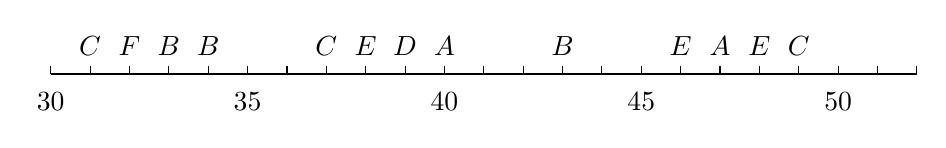
\begin{tikzpicture}

\draw (-5.5,0) -- (5.5,0);

\foreach \x in {-5.5,-5,...,5.5}
    \draw (\x,0) -- (\x,3pt);

\foreach \x [evaluate=\x as \timestamp using int((\x*2)+41)] in {-5.5,-3,...,5.5}
    \node at (\x,-1em) {$ \timestamp $};


\foreach \x/\eventtype in {
  -5/C,
  -4.5/F,
  -4/B,
  -3.5/B,
  -2/C,
  -1.5/E,
  -1/D,
  -0.5/A,
  1/B,
  2.5/E,
  3/A,
  3.5/E,
  4/C}
    \node at (\x,1em) {$ \eventtype $};

\end{tikzpicture}

\caption{A visual example of a sequence.}

\label{fig:event-sequence}
\end{figure}

Figure~\ref{fig:event-sequence} shows a visualization of a possible event sequence.

\begin{definition}
An \emph{episode} $ G $ is represented by a directed acyclic graph with labelled nodes, that is, $ G = (V, E, lab) $, where $ V = (v_1, \ldots, v_K) $ is the set of nodes, $ E $ is the set of directed edges, and lab is the function $ lab \colon V \rightarrow \Sigma $, mapping each node $ v_i $ to its event type.
\end{definition}

We write $ | \alpha | $ to mean the number of nodes in an episode's graph.

\begin{definition}
A node $ n $ in an episode graph is a \emph{descendant} of a node $ m $ if there is a path from $ m $ to $ n $. Conversely $ m $ is an \emph{ancestor} of $ n $ in that case.
\end{definition}

\begin{definition}
Given a sequence $ s $ and an episode $ G $ we say that $ s $ \emph{covers} G, or $ G $ \emph{occurs} in $ s $, if there is an injective map $ f $ mapping each node $ v_i $ to a valid index such that the node $ v_i $ in $ G $ and the corresponding sequence element $ s_{f(v_i)} $ have the same label: $ s_{f(v_i)} = lab(v_i) $; and that if there is an edge $ (v_i, v_j) $ in $ G $, then we must have $ f(v_i) < f(v_j) $. In other words, the parents of $ v_j $ must occur in $ s $ before $ v_j $. If the mapping $ f $ is surjective, that is, all events in $ s $ are used, we will say that $ s $ is an \emph{instance} of G.
\end{definition}

\begin{definition}
Given two episodes $ G $ and $ H $, we say that $ G $ is a \emph{subepisode} of $ H $, denoted $ G \subseteq H $, if the graph describing episode $ G $ is a subgraph of the graph describing episode $ H $.
\end{definition}

In this thesis, we'll be limiting ourselves to two subcategories of episodes:
\begin{itemize}
\item \textbf{Parallel episodes.} A parallel episode is an episode for which the set of edges is empty. As such, no constraints are placed on the order in which event types occur a sequence. An example is shown in figure~\ref{fig:episode-graphs-parallel}. In text we'll write parallel episodes by their event types using the following notation:
\begin{align*}
    \{ A, B, C \}
\end{align*}
by which we mean a parallel episode with three nodes, and the event types are A, B, and C. Note that though the notation reminds strongly of a mathematical set, it is not: a parallel episode $ \{ A, A, B, C \} $ is not equivalent to $ \{ A, B, C \} $.

\item \textbf{Serial episodes.} A serial episode is an episode for which the edges cause the nodes to have a strict order. That is, in any occurrence of a serial episode in a sequence, the event types appear in the same order. Figure~\ref{fig:episode-graphs-serial} shows an example.

Sometimes it is useful to describe serial episodes in their strict form, in which there is a direct edge between any two nodes. Figure~\ref{fig:episode-graphs-serial-strict} shows a strict episode which is equivalent to the episode in figure~\ref{fig:episode-graphs-serial}.

While serial episodes have a different graph in this form, their meaning is the same since they enforce the same order.

\end{itemize}

\begin{figure}

\begin{subfigure}[b]{\textwidth}
\centering
\begin{tikzpicture}

\node (n 1) [circly] at (-3,-3pt) {$ v_1 $};
\node (n 2) [circly] at (-1, 3pt) {$ v_2 $};
\node (n 3) [circly] at ( 1,-3pt) {$ v_3 $};
\node (n 4) [circly] at ( 3, 3pt) {$ v_4 $};

\end{tikzpicture}
\caption{parallel}
\label{fig:episode-graphs-parallel}
\end{subfigure}

\par\bigskip

\begin{subfigure}[b]{\textwidth}
\centering
\begin{tikzpicture}

\node (n 1) [circly] at (-3,0) {$ v_1 $};
\node (n 2) [circly] at (-1,0) {$ v_2 $};
\node (n 3) [circly] at ( 1,0) {$ v_3 $};
\node (n 4) [circly] at ( 3,0) {$ v_4 $};

\draw [->] (n 1) -- (n 2);
\draw [->] (n 2) -- (n 3);
\draw [->] (n 3) -- (n 4);

\end{tikzpicture}
\caption{serial}
\label{fig:episode-graphs-serial}
\end{subfigure}

\par\bigskip

\begin{subfigure}[b]{\textwidth}
\centering
\begin{tikzpicture}

\node (n 1) [circly] at (-3,0) {$ v_1 $};
\node (n 2) [circly] at (-1,0) {$ v_2 $};
\node (n 3) [circly] at ( 1,0) {$ v_3 $};
\node (n 4) [circly] at ( 3,0) {$ v_4 $};

\draw [->] (n 1) -- (n 2);
\draw [->] (n 2) -- (n 3);
\draw [->] (n 3) -- (n 4);

\draw [->] (n 1) to [bend left=30] (n 3);
\draw [->] (n 2) to [bend left=30] (n 4);
\draw [->] (n 1) to [bend left=30] (n 4);

\end{tikzpicture}

\caption{serial, strict}
\label{fig:episode-graphs-serial-strict}
\end{subfigure}

\caption{Episode graphs.}

\label{fig:episode-graphs}
\end{figure}

Because we only consider parallel and serial episodes, it is easy to represent an episode in a data structure---we don't need to explicitly store a graph with nodes and edges:
\begin{itemize}
\item Parallel episodes can be stored in an array, where each element is simply the event type of the episode. Strictly speaking, the order of the elements in the array doesn't matter, but in the implementation they will follow some order on the set of event types. In that way each parallel episode has a unique array representation. Figure~\ref{fig:parallel-representation} shows the representation visually.

\tikzset{circly/.style={draw,circle,minimum size=1cm},
    arraycell/.style={draw,rectangle,minimum size=1cm,node distance=0}}

\begin{figure}[h]
\centering

\begin{tikzpicture}

\node (n 1) [circly,label=above:$ C $] at (-3,-3pt) {$ v_1 $};
\node (n 2) [circly,label=above:$ A $] at (-1, 3pt) {$ v_2 $};
\node (n 3) [circly,label=above:$ B $] at ( 1,-3pt) {$ v_3 $};
\node (n 4) [circly,label=above:$ A $] at ( 3, 3pt) {$ v_4 $};

\node [left=of n 1] {episode graph};

\draw [->] (0,-1) -- node [left=0.5cm] {sort the event types into an array} +(0,-1.5);

\node (a 1) [arraycell] at (-2,-3.5) {$ A $};
\node (a 2) [arraycell,right=of a 1] {$ A $};
\node (a 3) [arraycell,right=of a 2] {$ B $};
\node (a 4) [arraycell,right=of a 3] {$ C $};

\end{tikzpicture}

\caption{A parallel episode's graph representation, with the label of each node shown above, and its array representation.}

\label{fig:parallel-representation}
\end{figure}

\item Serial episodes can also be stored in an array, but here the order of the elements is defined by the edges of the episode. That is, the event types are ordered according to a topological sort of the nodes. Figure~\ref{fig:serial-representation} shows this visually.
\end{itemize}

When discussing the algorithms we will mostly consider their array representation, and address their elements by array index by suffixing the episode identifier with the index in square brackets. For instance, $ \alpha [i] $ refers to the $ i $-th element of the array.

\begin{figure}
\centering

\begin{tikzpicture}

\node (n 1) [circly,label=above:$ A $] at (-3,0) {$ v_1 $};
\node (n 2) [circly,label=above:$ C $] at (-1,0) {$ v_2 $}
    edge [pre] (n 1);
\node (n 3) [circly,label=above:$ B $] at (1, 0) {$ v_3 $}
    edge [pre] (n 2);
\node (n 4) [circly,label=above:$ A $] at (3, 0) {$ v_4 $}
    edge [pre] (n 3);

\node [left=of n 1] {episode graph};

\draw [->] (0,-1) -- node [left=0.5cm,align=right] {store event types into array,\\preserving toplogical ordering} +(0,-1.5);

\node (a 1) [arraycell] at (-2, -3.5) {$ A $};
\node (a 2) [arraycell,right=of a 1] {$ C $};
\node (a 3) [arraycell,right=of a 2] {$ B $};
\node (a 4) [arraycell,right=of a 3] {$ A $};

\end{tikzpicture}

\caption{A serial episode's graph representation, with the label of each node shown above, and its array representation.}
\label{fig:serial-representation}
\end{figure}

\subsection{Association Rules}
\begin{definition}
Given two episodes $ G $ and $ H $ such that $ G \subset H $, we can express an \emph{association rule} $ G \Rightarrow H $. We call $ G $ the \emph{head} of the rule, and $ H $ the \emph{tail} of the rule.
\end{definition}

We present three methods to measure the frequency of an episode and the confidence of an association rule. In a later section, we implement a mining algorithm based on them.

\subsubsection{Fixed Windows}

The first frequency measure is based on windows of fixed length.

\begin{definition}
Given a window size $ \rho $ and a sequence $ s $, we define the \emph{fixed-window frequency} of an episode $ G $ in $ s $, denoted $ fr_f(G; s) $, to be the number of windows of size $ \rho $ in $ s $ covering the episode:
\begin{align*}
fr_f(G; s) = | \{ s[i, i + \rho - 1] | s[i, i + \rho - 1] \text{ covers } G \} |
\end{align*}
\end{definition}

\begin{definition}
Given a window size $ \rho $ and episodes $ X $ and $ Y $, such that $ X \subset Y $, we define the \emph{fixed-window confidence} of the association rule $ X \Rightarrow Y $, denoted $ c_f(X \Rightarrow Y) $, to be the ratio of their respective frequencies:
\begin{align*}
c_f(X \Rightarrow Y) = \frac{ fr_f(Y) }{ fr_f(X) }
\end{align*}
\end{definition}

\subsubsection{Minimal Windows}

\begin{definition}
Given a sequence $ s $ and an episode $ G $, a window $ s[a, b] $, is called a \emph{minimal window} of $ G $ in $ s $, if:
\begin{itemize}
\item $ len(s[a, b]) \leq \rho $, $ s[a, b] $, and
\item no proper subwindow of of $ s[a, b] $ covers $ G $.
\end{itemize}
We define beginning, end ... % TODO figure out definitions (inclusive-exclusive end-timestamp)

We denote the set of all minimal windows of $ G $ in $ s $ with $ mw(G; s) $, or simply $ mw(G) $ if $ s $ is known from the context. Given a set of minimal windows $ W $, we define a function $ dis(W) $ to be equal to 1 if all windows in $ W $ are pairwise disjoint, and 0 otherwise.
\end{definition}

\begin{definition}
The \emph{disjoint-window frequency} of an episode $ G $ in a sequence $ s $, denoted $ fr_m(G) $, is defined as the maximal number of non-overlapping minimal windows within $ s $ that contain episode $ G $. Formally:
\begin{align*}
fr_m(G) = \text{max} \{ | W | \mid W \subseteq mw(G) \wedge dis(W) = 1 \}
\end{align*}
\end{definition}

\begin{definition}
Given episodes $ X $ and $ Y $, such that $ X \subset Y $, and a minimal window $ s[a, b] $ of episode $ X $. Assume there exists a minimal window $ s[c, d] $ of $ Y $ such that $ c \leq a $ and $ b \leq d $, then we define the \emph{minimal-extensibility} of occurrence $ s[a, b] $ of $ X $ into an occurrence of $ Y $ as
\begin{align*}
ext_m(s[a, b], X, Y) = 1
\end{align*}
If there exists no such minimal window of $ Y $, we define $ ext_m(s[a, b], X, Y) = 0 $.
\end{definition}

\subsubsection{Weighted Minimal Windows}

\begin{definition}
The \emph{total weight} of a set of windows $ W $ in a sequence $ s $, denoted $ tw(W) $, is defined as
\begin{align*}
tw(W) = \sum_{w \in W}{\frac{1}{len(w)}}
\end{align*}
The \emph{weighted-window frequency} of an episode $ G $ in a sequence $ s $, denoted $ fr_w(G) $, is defined as
\begin{align*}
fr_w(G) = \text{max} \{ tw(W) | W \subseteq mw(G), dis(W) = 1 \}
\end{align*}
\end{definition}
